% slides.tex
% A demo of the Prosper documentclass for \LaTeX
%
% The layout and colors in this demo are designed to look best with
% UMBC's Prosper styles.  The demo should compile with any other Prosper
% style, however the results will not be ideal because slide dimensions,
% fonts sizes and color pallets vary widely from style to style.
% 
% When you create your own Prosper document, first you pick a style,
% then lay out the contents to fit that specific style.
% 
% You may want to have a look at the tutorial in:
%     http://www.math.umbc.edu/~rouben/prosper/
% 
% Rouben Rostamian <rostamian@umbc.edu>
% January 2003

\documentclass[pdf,slideColor,colorBG]{prosper}
\ptsize{9}




% If using a umbc* style, we add a logo and navigation icons 
% The navigation icons look like this:   " <--   O  -->"
% In the Acrobat Reader, if you click on an icon by the left mouse button:
%   o the left icon takes you to the first slide
%     (it's equivalent to Control-Shift-PageUp)
%   o the right icon takes you to the last slide
%     (it's equivalent to Control-Shift-PageDown)
%   o the middle icon takes you to the last viewed slide.  Use it to
%     return to the previous page after a hyperlink jump.
%     (it's equivalent to Control-LeftArrow)
%
% REMOVE THE FOLLOWING BLOCK OF LINES entirely if you don't care for the UMBC
% logo and navigation icons.
%\usepackage{ifthen}
%ifthenelse{\not\isundefined{\umbclogo}}
\usepackage{amssymb}
\usepackage{amsthm}
%\usepackage{color}
\usepackage[fleqn]{amsmath}
\usepackage[ruled,vlined]{algorithm2e}


\title{Learning Coordinate Covariances via Gradients} 
\author{Sayan Mukherjee$^1$ and  Ding-Xuan Zhou$^2$}
\email{sayan@stat.duke.edu$^1$, mazhou@cityu.edu.hk$^2$}
\institution{{\blue Institute for Genome Sciences and Policy$^1$} \\
{\blue Institute of Statistics and Decision Sciences$^1$} \\  
{\blue Duke University} \\
{\red Department of Mathematics$^2$}\\
{\red City University of  Hong Kong$^2$}
}



% The following block of lines are specific to this document.
% DONT'T COPY THEM TO YOUR documents if you don't need them.
\newcommand{\pd}[2]{\frac{\partial #1}{\partial #2}}    % partial derivatives
\renewcommand{\div}{\mathop\mathrm{div}\nolimits}       % divergence
\newcommand{\header}[1]{\textbf{\textsl{{\blue #1}}}}   % a convenience macro
\newcommand{\highlight}[1]{% highlight text as with a yellow marker
        \psframebox[fillstyle=solid,fillcolor=yellow,linestyle=none]{#1}%
}
\renewcommand{\P}{\text{P}}
\renewcommand{\R}{{\rm I\!R}}
\newcommand{\pr}{{\rm I\!P}}
\newcommand{\E}{{\rm I\!E}}
\newcommand{\N}{{\rm I\!N}}
\newtheorem{conj}{Conjecture}
\newtheorem{countex}{Counterexample}
\newtheorem{prop}{Proposition}
\newtheorem{thm}{Theorem}
\newtheorem{cor}{Corollary}
\newtheorem{defn}{Definition}
\newtheorem{lem}{Lemma}
%\renewcommand{\ell}{l}
\newcommand{\SSS}{\scriptscriptstyle}
\newcommand{\MC}{\multicolumn}
\newcommand{\cT}{\ensuremath{{\cal T}}}
\newcommand{\z}{\ensuremath{\pi}}
\newcommand{\sZ}{\ensuremath{\Pi}}
\newcommand{\bz}{\ensuremath{\mbox{\boldmath$\pi$}}}
\newcommand{\Pperm}{\ensuremath{{\hat{P}}}}
\newcommand{\Pnull}{\ensuremath{{{P}_{\mbox{null}}}}}
\newcommand{\bx}{\ensuremath{{\bf x}}}
\newcommand{\bzz}{\ensuremath{{\bf z}}}
% set up hyperlink colors
\hypersetup{colorlinks=true,anchorcolor=green,linkcolor=red,menucolor=cyan}
%%================Math symbol ============================
\def\nn{{\mathbb N}}
\def\zz{{\mathbb Z}}
\def\rr{{\mathbb R}}
\def\rn{{\mathbb R}^n}

%%=============Display style operator =====================
\def\dsum{\displaystyle\sum}
\def\dint{\displaystyle\int}
\def\dfrac{\displaystyle\frac}
\def\dsup{\displaystyle\sup}
\def\dinf{\displaystyle\inf}
\def\dmin{\displaystyle\min}
\def\dlim{\displaystyle\lim}


%%=========Greek Letters =================
\def\gep{\varepsilon}
\def\ga{\alpha}
\def\gb{\beta}
\def\gs{\sigma}
\def\gd{\delta}
\def\gl{\lambda}
\def\gga{\gamma}
\def\gS{\Sigma}
\def\gD{\Delta}

%============ Special notations ===============
\newcommand{\set}[1]{\left\{#1\right\}} % set
\def\E{{\mathcal E}} % generalization error
\def\H{{\mathcal H}} % hypothesis space
\def\H{{\mathcal H}} % hypothesis space
\def\N{{\mathcal N}} % covering number
\def\D{{\mathcal D}} % regularization error
\def\bz{{\bf z}} % sample
\DeclareMathOperator\sgn{sgn} % sign function
\DeclareMathOperator\Span{span} % linear span
\DeclareMathOperator\Diam{Diam} % diameter of a set
\DeclareMathOperator\bE{\mathbb E} % expectation
\DeclareMathOperator*\prob{{\bf P}rob} % probability in product space






\Logo{% \umbclogo
        \hspace{5cm}
        \tiny
        \Acrobatmenu{FirstPage}{$\rule{0.20ex}{1ex}\!\!\blacktriangleleft$}
        \qquad
        \Acrobatmenu{GoBack}{$\circlearrowright$}
        \qquad
        \Acrobatmenu{LastPage}{$\blacktriangleright\!\!\rule{0.20ex}{1ex}$}
}

% The "pst-node" package is used in the slide titled:
%           "Boundary conditions derived from symmetries".
% Most users won't need this.
% DON'T COPY THIS TO YOUR documents unless you know what it does.


\begin{document}

%-------------------------------------------------------------------- Slide --

\maketitle

%-------------------------------------------------------------------- Slide --

\overlays{7}{
\begin{slide}{Overview}

{\small

\begin{itemize}

\fromSlide*{1}{
\item Motivation of problem
}

\fromSlide*{2}{
\item Tikhonov regularization
}

\fromSlide*{3}{
\item Learning the gradient}

\fromSlide*{4}{
\item A representer theorem
}

\fromSlide*{5}{
\item A reduced matrix algorithm
}

\fromSlide*{6}{
\item Convergence of the estimate of the gradient}

\fromSlide*{7}{
\item Applications to simulated and real data}

 
\end{itemize}

}
\end{slide}

}

%-------------------------------------------------------------------- Slide --


\overlays{3}{
\begin{slide}{Motivation}
{\small

\fromSlide*{1}{
Classification and regression of high dimensional data given few
samples. \\
The ``large p, small n'' paradigm. \\
Tikhonov regularization/shrinkage estimators (for example SVMs)
have been successful. \\
}

\vspace{.2in}
\fromSlide*{2}{
In a number of problems classical questions from statistical linear
modeling have been revived
\begin{itemize}
\item variable saliency/significance
\item coordinate covariation
\end{itemize}
However in the ``large p, small n'' paradigm. \\
}
\vspace{.2in}


\fromSlide*{3}{
We formulate the problem of learning coordinate covariation 
and relevance in the framework of Tikhonov regularization or
shrinkage estimation.
}
}

\end{slide}
}
%-------------------------------------------------------------------- Slide --



\overlays{5}{
\begin{slide}{Tikhonov regularization}


{\small
\fromSlide*{1}{
$X \subseteq \R^n$ is a compact metric space and $Y \subseteq \R$ \\
a sample ${\bf z}=\bigl\{(x_i, y_i)\bigr\}_{i=1}^m \in (X\times
Y)^m$ \\
} 
\vspace{.1in}
\fromSlide*{2}{
a hypothesis space ${\mathcal H}$ is a set of functions
$f: X \rightarrow Y \subset \R$ \\}
\vspace{.1in}
\fromSlide*{3}{
a loss functional $V(f(x),y): \R \times \R \to \R_+$ \\}
\vspace{.1in}
\fromSlide*{4}{
a penalty or smoothness functional $\Omega: {\mathcal H} \to \R_+$ on
${\mathcal H}$ for example $\Omega(f) = \|f\|_K^2$ \\}
\vspace{.1in}
\fromSlide*{5}{
\begin{displaymath}
f_{\bf z}^V = \arg\min_{f\in {\cal H}} \Big\{ \frac{1}{m}
   \sum_{i=1}^m V(y_i, f(x_i)) + \gl \Omega(f)\Big\}
\end{displaymath}
where $\lambda >0$
}


}
\end{slide}
}

%-------------------------------------------------------------------- Slide --


\overlays{4}{
\begin{slide}{Reproducing Kernel Hilbert Spaces}


{\small
\onlySlide*{1}{
 $K: X\times X \to \R$ be continuous, symmetric and positive
semidefinite is a Mercer kernel, for example 
$$K(w,v) = \frac{1}{\sqrt{2 \pi} \sigma} \exp(-\|u-v\|^2 /2
\sigma^2)$$ \\
}


\vspace{.1in}
\fromSlide*{2}{RKHS is the linear span
$${\mathcal H}_{K} = \mbox{span}\{K_x := K(x, \cdot): \, x \in X\}$$
$$\langle K_v, K_u\rangle_K = K(u, v)$$
}

\vspace{.1in}
\fromSlide*{3}{
reproducing property
$$\langle K_x, f\rangle_{K} = f(x), \qquad \forall x\in X, f\in
{\mathcal H}_K$$ \\}

\vspace{.1in}
\fromSlide*{4}{
\begin{displaymath}
f_{\bf z}^V = \arg\min_{f\in {\cal H}_K} \Big\{ \frac{1}{m}
   \sum_{i=1}^m V(y_i, f(x_i)) + \gl \|f\|_K^2 \Big\}
\end{displaymath}
$$f_{\bf z}^V(x) =\sum_{i=1}^m c_i K(x_i,x)$$
optimization over $\{c_i\}_{i=1}^m \in \R^m$ 
}




}
\end{slide}
}

%-------------------------------------------------------------------- Slide --



\overlays{3}{
\begin{slide}{The regression function}


{\small

\fromSlide*{1}{
the joint
$${\bf z}=\bigl\{(x_i, y_i)\bigr\}_{i=1}^m \sim \rho(x,y) $$}

\vspace{.1in}

\fromSlide*{2}{
assume $V(y, f(x)) = (y-f(x))^2$ \\
the regression function
$$f_\rho (x) = \int_Y y d\rho (y|x), \qquad x\in X$$
}
\vspace{.1in}

\fromSlide*{3}{
Convergence: as $\lambda =\lambda(m) \to 0$ as $m\to \infty$
$$\|f_{\bf z}^V-f_\rho\|_{\rho} \rightarrow 0$$
}

}
\end{slide}
}



%-------------------------------------------------------------------- Slide -
\overlays{3}{
\begin{slide}{Classification}


{\small

\fromSlide*{1}{

$Y=\{-1, 1\}$ and $\hbox{sgn}(f): X \to Y$ \\
loss function: $V(f(x),y) = \phi(y f(x)) := \log \bigl(1 + e^{-y f(x)}\bigr)$
\begin{displaymath}
f_{\bf z}^V = \arg\min_{f\in {\cal H}_K} \Big\{ \frac{1}{m}
   \sum_{i=1}^m \log \bigl(1 + e^{-y_i f(x_i)}\bigr)  + \gl \|f\|_K^2 \Big\}
\end{displaymath}
}

\vspace{.1in}

\fromSlide*{2}{
classification error
$${\cal R}(\hbox{sgn}(f))=\hbox{Prob}\{\hbox{sgn}(f(x)) \not= y\}$$
the Bayes (optimal) rule  
$$\hbox{sgn}(f_\rho)$$
}


\vspace{.1in}

\fromSlide*{3}{
Convergence: as $\lambda =\lambda(m) \to 0$ as $m\to \infty$ \\
$$ {\cal R}(\hbox{sgn}(f_{\bf z}^V)) \rightarrow {\cal R}(\hbox{sgn}(f_\rho))$$
}

}
\end{slide}
}






%-------------------------------------------------------------------- Slide -
\overlays{2}{
\begin{slide}{Learning the gradient}


{\small

\fromSlide*{1}{
$x=(x^1, x^2, \ldots, x^n)^T \in \R^n$ and the gradient of 
$f_\rho$
$$\nabla f_\rho =\left(\frac{\partial f_\rho}{\partial x^1},\; \ldots,\;
\frac{\partial f_\rho}{\partial x^n}\right)^T$$
}

\vspace{.1in}

\fromSlide*{2}{
use of the gradient
\begin{itemize}
\item variable selection: $\left\|\frac{\partial f_\rho}{\partial x^i}\right\|$
\item coordinate covariation: $\left \langle \frac{\partial f_\rho}{\partial x^i}, \frac{\partial f_\rho}{\partial x^j} \right \rangle$
\end{itemize}
}



}
\end{slide}
}


%-------------------------------------------------------------------- Slide -
\overlays{3}{
\begin{slide}{Formulating the algorithm}


{\small

\fromSlide*{1}{
Taylor expanding $f(u)$ around $x$ 
$$f(u) \approx f(x) + \int_{\Delta x \in \Gamma_x} \langle \nabla f, \Delta x\rangle,$$
where the inner product and neighborhood $\Gamma_x$ depend on the
problem setting}


\vspace{.1in}

\onlySlide*{2}{
manifold setting: $\rho_X$ is concentrated on a
manifold $\cal M$
$$f(u) \approx f(x) + \int_{\Delta x \in {\cal M}_x}
\langle \nabla_{\cal M} f, \Delta x\rangle,$$ 
where ${\Delta x \in {\cal M}_x}$ and the inner product is
$L_2$ over the manifold
}

\vspace{.2in}

\fromSlide*{3}{
various algorithms can be realized by a robust mininimization of the error 
$f(u)$ and its expansion 
$$f(x)+\int_{\Delta x \in  \Gamma_x} \langle \nabla f, \Delta x\rangle
\approx f(x) + \nabla f(x) \cdot (u-x) \mbox{     for } u\approx x$$
}



}
\end{slide}
}

%-------------------------------------------------------------------- Slide -

\overlays{4}{
\begin{slide}{Elements for algorithm}


{\small

\onlySlide*{1}{
loss function for regression: on sample points $x=x_i, u=x_j$
$$\bigl(f(u)- f(x) - \nabla f(x) \cdot (u-x) \bigr)^2 :=
\bigl(y_i-y_j+ \vec f (x_i)\cdot (x_j-x_i)\bigr)^2 \mbox{     for }
x_i \approx x_j$$
where $x_i\approx x_j$ given by  weights: $w_{i, j}>0$}



\onlySlide*{2}{
loss function for classification: on sample points $x=x_i, u=x_j$
and convex function $\phi$ (logistic)
$$\phi\biggl(y_i \bigl(y_j+ \vec f (x_i)\cdot (x_i -x_j)\bigr)\biggr)
 \mbox{     for } x_i \approx x_j$$
where $x_i\approx x_j$ given by  weights: $w_{i, j}>0$}


\fromSlide*{3}{
loss function for regression: on sample points $x=x_i, u=x_j$
$$\bigl(f(u)- f(x) - \nabla f(x) \cdot (u-x) \bigr)^2 :=
\bigl(y_i-y_j+ \vec f (x_i)\cdot (x_j-x_i)\bigr)^2 \mbox{     for }
x_i \approx x_j$$
where $x_i\approx x_j$ given by  weights: $w_{i, j}>0$

\vspace{.1in}

weights: a natural choice is a Gaussian
$$w_{i, j}=w_{i, j}^{(s)}=\frac{1}{s^{n+2}} e^{-\frac{|x_i-x_j|^2}{2s^2}} =w(x_i - x_j), \qquad i, j =1, \ldots, m$$
}


\vspace{.1in}
\fromSlide*{4}{
regularization: $\H_K^n$ is an $n$-fold of ${\cal H}_K$
and $\vec f =(f_1, f_2, \ldots,f_n)^T$ with $f_\ell \in \H_K$ \\
$$\langle \vec f, \vec g \rangle_K =\sum_{\ell =1}^n \langle
f_\ell, g_\ell \rangle_K \mbox{   and  } \|\vec f\|_K^2 =\sum_{\ell=1}^n
\|f_\ell\|_K^2$$
}



}
\end{slide}
}
%-------------------------------------------------------------------- Slide -


\overlays{2}{
\begin{slide}{Gradient algorithms}


{\small

\fromSlide*{1}{
\begin{defn}
The least-square type learning algorithm is defined for the sample
$\bz \in Z^m$ as
\begin{displaymath}
 \vec f_{\bz, \gl}: =\arg\min_{\vec f \in\H_K^n}
\biggl\{\frac{1}{m^2}\sum_{i, j=1}^m w_{i, j}^{(s)}
\biggl(y_i-y_j+ \vec f (x_i)\cdot (x_j-x_i)\biggr)^2 + \gl\|\vec
f\|_K^2\biggr\},
\end{displaymath} where $\lambda, s$ are two positive constants
called the {\it regularization parameters}.
\end{defn}
}


\vspace{.3in}

\fromSlide*{2}{
\begin{defn}
The regularization scheme for classification is defined for the
sample $\bz \in Z^m$ as
\begin{displaymath}
 \vec f_{\bz, \gl} =\arg\min_{\vec f \in\H_K^n}
\biggl\{\frac{1}{m^2}\sum_{i, j=1}^m w_{i, j}^{(s)} \phi
\biggl(y_i \bigl(y_j+ \vec f (x_i)\cdot (x_i -x_j)\bigr)\biggr) +
\gl\|\vec f\|_K^2\biggr\}.
\end{displaymath}
\end{defn}
}

}
\end{slide}
}




%-------------------------------------------------------------------- Slide --
\overlays{2}{
\begin{slide}{Remark}


{\small

\fromSlide*{1}{
Why not estimate $f_\rho$ and then take partial derivatives ?
}

\vspace{.2in}

\fromSlide*{2}{
When we obtain an approximation of $f_\rho$ it is in a particular
RKHS.\\
However, its partial derivatives are not.\\ 
Hence, there is no natural ways to find the correlations. \\
For example for the Gaussian kernel, there are no natural inner
products among its partial derivatives, especially when there are no 
natural coordinates for the underlying manifold.}

}
\end{slide}
}

%-------------------------------------------------------------------- Slide -


\overlays{2}{
\begin{slide}{Representer theorems}


{\small

\onlySlide*{1}{
For both classification and regression
$$\vec f_{\bz,\gl}(x) =\sum_{i=1}^m c_{i,\bz} K({x_i},x),$$
where $c_{i,\bz} \in \R^n$.
}



\fromSlide*{2}{
For regression
\begin{thm}
For $i=1,\ldots,m,$ let $B_i$
\begin{displaymath}\label{BY}
B_i=\sum_{j=1}^m w_{i, j} (x_j-x_i) (x_j-x_i)^T \in\rr^{n\times
n}, \quad Y_i =\sum_{j=1}^m w_{i, j} (y_j-y_i)(x_j-x_i) \in\rr^n.
\end{displaymath}
Then 
$$\vec f_{\bz, \gl}(x) =\sum_{i=1}^m c_{i, \bz} K({x_i},x)$$ 
with
$c_{\bz}=(c_{1,\bz}^T, \ldots, c_{m, \bz}^T)^T \in\rr^{m n}$
satisfying the linear system 
\begin{displaymath}\label{linsysone}
\biggl\{ m^2 \gl I_{mn}
   + \hbox{diag}\{B_1, B_2, \cdots, B_m\}
   \bigl[K(x_i,x_j)I_{n}\bigr]_{i,j=1}^m
\biggr\} c =(Y_1^T, Y_2^T, \ldots, Y_m^T)^T.
\end{displaymath}
\end{thm}

\vspace{.1in}
The above is a linear system of size $mn \times mn$ which
is prohibitive if $n >> m$.

}

}
\end{slide}
}

%-------------------------------------------------------------------- Slide -


\overlays{2}{
\begin{slide}{Reducing the matrix size}


{\small

\onlySlide*{1}{
Each term in the summation defining $B_i$ is a rank one matrix. \\
Hence the rank of the $n\times n$ matrix $B_i$ is at most $m$. \\
This allows us to reduce the system to $(dm)\times (dm)$ with $d\leq
m-1$. \\

\vspace{.1in}
Denote $V_{\bf x} =\hbox{span}\{x_j - x_m\}_{j=1}^{m-1}$, 
the subspace of $\rr^n$ generated by the vectors $\{x_j -x_m\}$.
}


\fromSlide*{2}{
\begin{thm}\label{reduce}
Let an $n\times d$ matrix $V=(V_1, \ldots, V_d)$ have linearly
independent column vectors and its column space
$\hbox{span}\{V_\ell\}_{\ell=1}^d$ contains $V_{\bf x}$. Write
$$x_j - x_m =\sum_{\ell=1}^d \widetilde{x}_j^\ell V_\ell = V
\widetilde{x}_j$$ 
with $\widetilde{x}_j \in\rr^d$ for each $j$.
Then 
$$\vec f_{\bz, \gl}(x)=\sum_{i=1}^m \bigl\{\sum_{\ell=1}^d
\widetilde{c}_{i, \bz}^\ell V_\ell\bigr\} K({x_i},x)$$ 
with
$\widetilde{c}_{\bf z}=(\widetilde{c}_{1, \bz}^T, \ldots,
\widetilde{c}_{m, \bz}^T)^T \in\rr^{m d}$ satisfying
\begin{displaymath}\label{linsystwo}
\biggl\{ m^2 \gl I_{md}
   + \mbox{diag}\{\widetilde{B}_1, \widetilde{B}_2, \cdots, \widetilde{B}_m\}
   \bigl[K(x_i,x_j)I_{d}\bigr]_{i,j=1}^m
\biggr\} \widetilde{c} =(\widetilde{Y}_1^T, \widetilde{Y}_2^T,
\ldots, \widetilde{Y}_m^T)^T.
\end{displaymath}
where $\widetilde{B}_i=\sum_{j=1}^m w_{i, j} (\widetilde{x}_j-
\widetilde{x}_i) (x_j-x_i)^T V \in\rr^{d\times d}, \quad
\widetilde{Y}_i =\sum_{j=1}^m w_{i, j} (y_j-y_i)(\widetilde{x}_j-
\widetilde{x}_i) \in\rr^d$.
\end{thm}
}

}
\end{slide}
}

%-------------------------------------------------------------------- Slide -


\begin{slide}{Convergence to the gradient}


{\small
\begin{prop}\label{simplerates}
Assume $|y| \leq M$ almost surely. Suppose that for some $0<\tau
\leq 2/3, c_\rho >0$, the marginal distribution $\rho_X$ satisfies
\begin{displaymath}\label{boundary}
\rho_X \bigl(\{x\in X: \inf_{u\not\in X}  |u-x| \leq s\}\bigr)
\leq c_\rho^2 s^{4 \tau}, \qquad \forall s>0, \end{displaymath} and
the density $p(x)$ of $d \rho_X (x)$ exists and satisfies
\begin{displaymath}\label{density}
\sup_{x\in X} p(x) \leq c_\rho, \quad |p(x) - p(u)| \leq c_\rho
|u-x|^\tau, \qquad \forall u, x\in X.
\end{displaymath}
Choose $\gl =\gl(m) = m^{-\frac{\tau}{n + 2 + 3 \tau}}$ and
$s=s(m) = (\kappa c_\rho)^{\frac{2}{\tau}} m^{-\frac{1}{n + 2 + 3
\tau}}$. If $\nabla f_\rho \in {\cal H}_K^n$ and the kernel $K$ is
$C^3$, then there is a constant $C_{\rho, K}$ such that for any
$0<\delta <1$ and $m\geq 1$, with confidence $1-\delta$, we have
\begin{displaymath}\label{firstrates} \|\vec f_{\bz, \gl} -\nabla
f_\rho\|_\rho \leq C_{\rho, K} \log \biggl({2 \over \delta}\biggr)
\biggl(\frac{1}{m}\biggr)^{\frac{\tau}{2(n + 2 + 3 \tau)}}.
\end{displaymath}
\end{prop}

}
\end{slide}

%-------------------------------------------------------------------- Slide -

\overlays{2}{
\begin{slide}{Quantities of interest}


{\small
\fromSlide*{1}{
\begin{defn}
The relative magnitude of the norm for the variables is defined as
$$s_\ell^{\rho} = \frac{\|\bigl(\vec f_{{\bf z}, \gl}\bigr)_\ell\|_K}
{\bigl(\sum_{j=1}^n \|\bigl(\vec f_{{\bf z},
\gl}\bigr)_j\|_K^2\bigr)^{1/2}}, \qquad \ell =1, \ldots, n.$$
\end{defn}
}

\vspace{.2in}

\fromSlide*{2}{
\begin{defn}
The {\bf empirical gradient matrix} (EGM), $F_{\bf z}$, is the
$n\times m$ matrix whose columns are $\vec{f}_{{\bf z}, \gl}(x_j)$
with $j=1, \ldots, m$. The {\bf empirical covariance matrix}
(ECM), $\Xi_{\bf z}$, is the $n \times n$ matrix of inner products
of the gradient between two coordinates
$$\mbox{Cov}(\vec{f}_{{\bf z}, \gl}) :=  \left[\langle\bigl(\vec
  f_{{\bf z}, \gl}\bigr)_p,\bigl(\vec f_{{\bf z}, \gl}\bigr)_q
\rangle_K \right]_{p, q =1}^n = \sum_{i,j=1}^m c_{i,{\bf z}}
c_{j,{\bf z}}^T K(x_i,x_j).$$
\end{defn}
}

}
\end{slide}

}


%-------------------------------------------------------------------- Slide -


\overlays{4}{
\begin{slide}{Simulated data}


{\small
\onlySlide*{1}{
Construct a function in an $n=80$ dimensional space which
consists of three linear functions over different partitions of
the space. So $\{(x_i,y_i)\}_{i=1}^{30}$ with $y \in \R$ and 
$x \in \R^{80}$.}
 
\onlySlide*{2}{
$\{x_i\}_{i=1}^{30}$ partition the space
\begin{enumerate}
\item{For samples $\{x_i\}_{i=1}^{10}$}
$$x^{j} = \mathcal{N}(1, \sigma_x), \ \hbox{for } j=1, \ldots, 10;
\qquad  x^{j} = \mathcal{N}(0,\sigma_x), \ \hbox{for } j=11, \ldots, 80. $$
\item{For samples $\{x_i\}_{i=11}^{20}$}
$$x^{j} = \mathcal{N}(1, \sigma_x), \ \hbox{for } j=11, \ldots, 20;
\qquad  x^{j} = \mathcal{N}(0,\sigma_x), \ \hbox{for } j=1, \ldots, 10,
21, \ldots, 80. $$
\item{For samples $\{x_i\}_{i=21}^{30}$}
$$x^{j} = \mathcal{N}(-1, \sigma_x), \ \hbox{for } j=41, \ldots, 50;
\qquad  x^{j} = \mathcal{N}(0,\sigma_x), \ \hbox{for } j=1, \ldots, 40, 51, \ldots,  80. $$
\end{enumerate}
}

\onlySlide*{3}{
Vectors corresponding to different linear functions over partitions
\begin{eqnarray*}
w_1 & = & 2 + .5 \sin(2 \pi i/10) \, \, \, \mbox{for } i=1,...,10 \, \,
\, \mbox{ and } 0 \, \, \mbox{ otherwise},\\
 w_2 & = & -2 - .5 \sin(2 \pi i/10) \, \, \, \mbox{for } i=11,...,20 \, \,
\, \mbox{ and } 0 \, \, \mbox{ otherwise},\\
 w_3 & = & -2 - .5 \sin(2 \pi i/10) \, \, \, \mbox{for } i=41,...,50 \, \,
\, \mbox{ and } 0 \, \, \mbox{ otherwise}.
\end{eqnarray*}
}

\onlySlide*{4}{
$\{y_i\}_{i=1}^{30}$ 
\begin{enumerate}
\item{For samples $\{y_i\}_{i=1}^{10}$
$$y_i = x_i \cdot w_1  + \mathcal{N}(0,\sigma_y),$$}
\item{For samples $\{y_i\}_{i=11}^{20}$
$$y_i = x_i \cdot w_2  + \mathcal{N}(0,\sigma_y),$$}
\item{For samples $\{y_i\}_{i=21}^{30}$
$$y_i = x_i \cdot w_3  + \mathcal{N}(0,\sigma_y).$$}
\end{enumerate}
}



}
\end{slide}

}

%-------------------------------------------------------------------- Slide -


\overlays{3}{
\begin{slide}{Simulated data}


{\small

\onlySlide*{1}{
\begin{center}
\centerline{
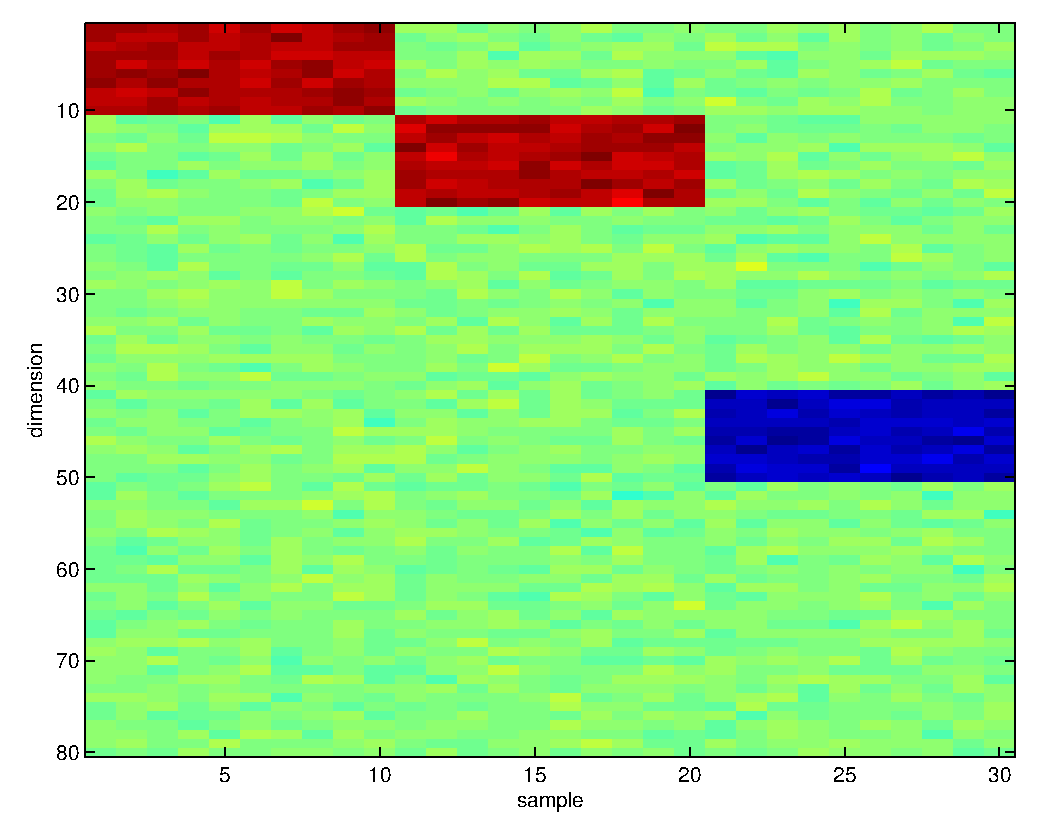
\includegraphics[scale=0.3]{xval.eps}
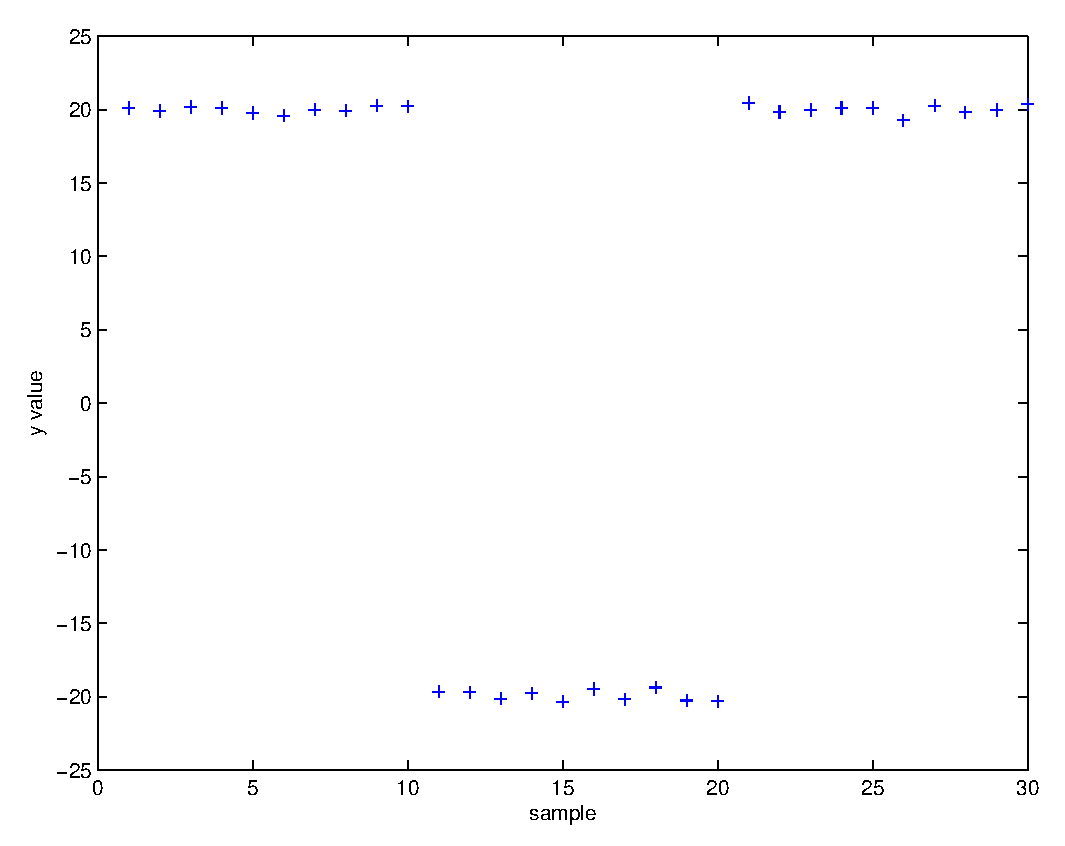
\includegraphics[scale=0.3]{yval.eps}
}
\end{center}
}

\onlySlide*{2}{
\begin{center}
\centerline{
\includegraphics[scale=0.3]{norm.eps}
}
\end{center}
}

\onlySlide*{3}{
\begin{center}
\centerline{
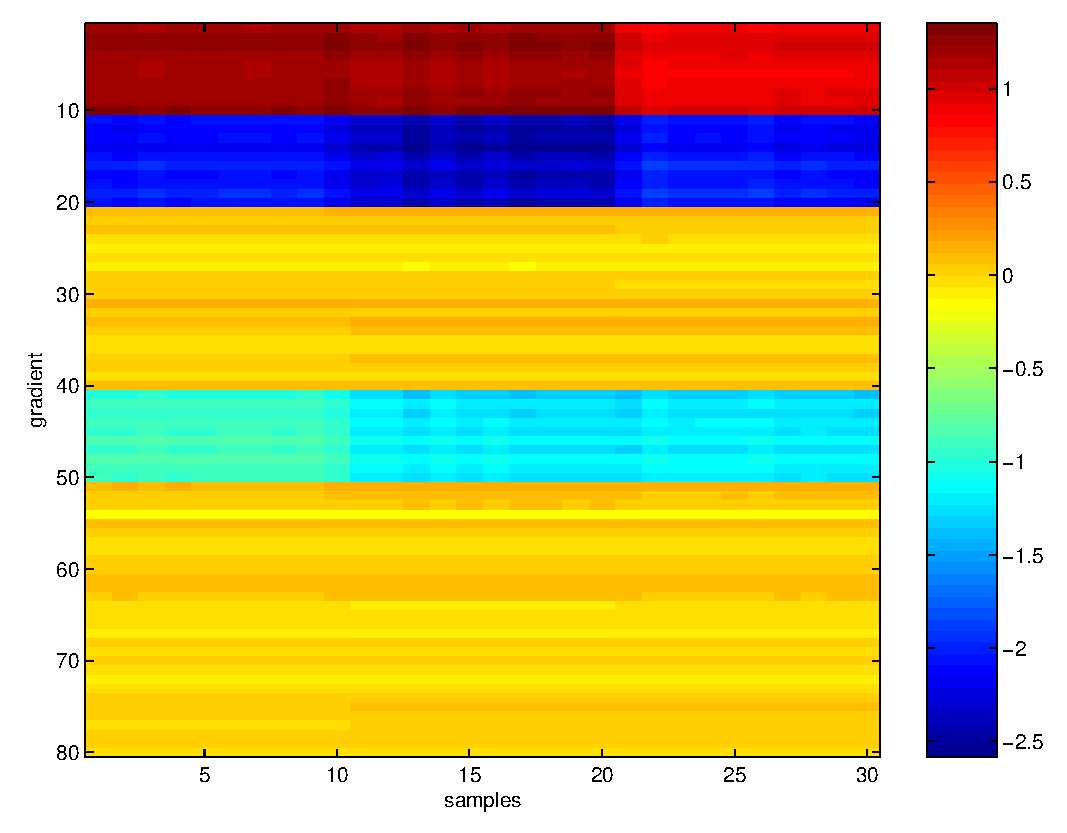
\includegraphics[scale=0.3]{gradient.eps}
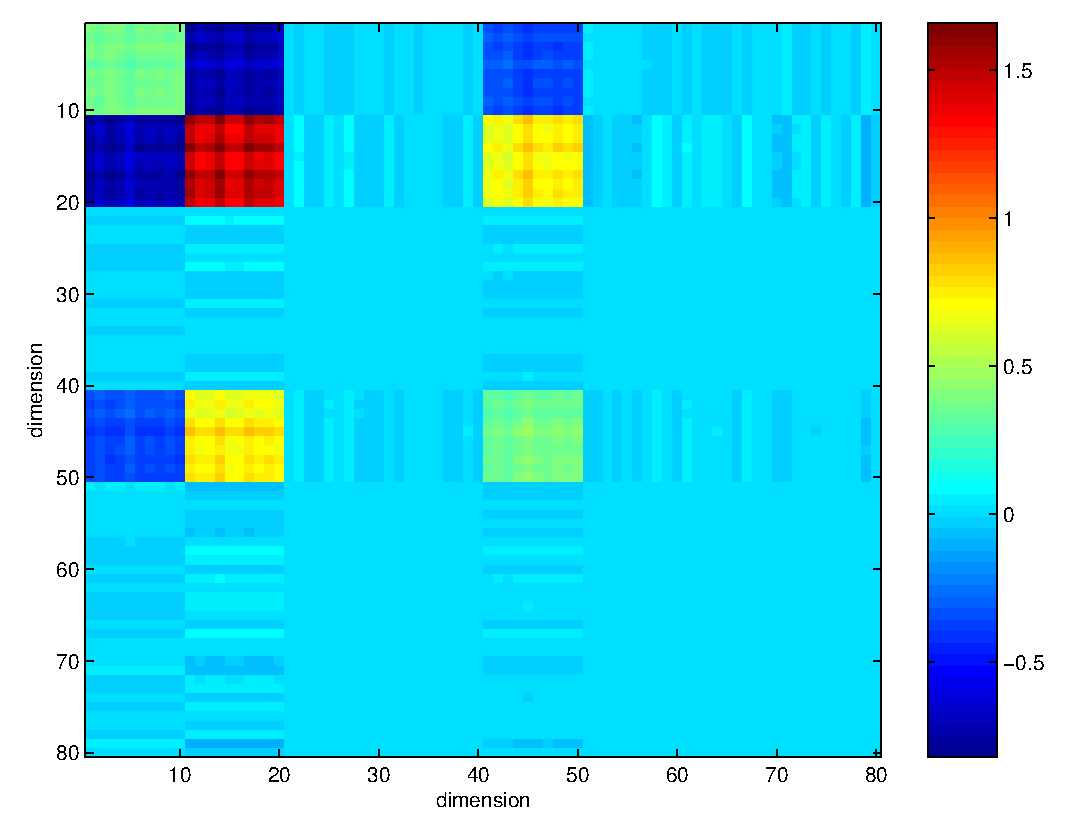
\includegraphics[scale=0.3]{covar.eps}
}
\end{center}
}


}
\end{slide}

}


%-------------------------------------------------------------------- Slide -


\overlays{3}{
\begin{slide}{Gene expression data}


{\small

\fromSlide*{1}{
Expression (number of copies of mRNA) for $7,129$ genes and ESTs
were measured over $73$ patients with either AML (myeloid leukemia)
or ALL (lymphoblastic leukemia) \\
\vspace{.1in}
$\{(x_i,y_i) \}_{i=1}^{73}$ with $x \in \rr^{7129}$ and $y \in \{-1,1\}$ \\
\vspace{.1in}
$38$ samples were used for the training set, $35$ for the test set
}
\vspace{.3in}

\fromSlide*{2}{

\centerline{
\begin{tabular}{||l|l|l|l|l|l|l|l|l|l|l||r} \hline
genes ({\cal S}) & 5 & 55 & 105 & 155 & 205 & 255 & 305 & 355 &
405 & 455
\\ \hline test errors & 1 & 3 & 2 & 1 & 1 & 1 & 1 & 1 & 1 & 1 \\
\hline
\end{tabular}}}

}

\end{slide}

}

%-------------------------------------------------------------------- Slide -


\overlays{3}{
\begin{slide}{Decay of norms}


{\small

\onlySlide*{1}{

The decay of $s_{(\ell)}^{\rho}$ is a measure of how many features
are significant }

\onlySlide*{2}{
Fisher score:
$$t_\ell =
\frac{|\hat{\mu}_\ell^{\tiny \mbox{AML}}-\hat{\mu}_\ell^{\tiny \mbox{ALL}}|}{\hat{\sigma}_\ell^{\tiny \mbox{AML}}+\hat{\sigma}_\ell^{\tiny \mbox{ALL}}},$$
$$s_\ell^{F} = \frac{t_\ell}{\bigl(\sum_{p=1}^n t_p^2\bigr)^{1/2}}$$
}


\onlySlide*{3}{
\begin{center}
\centerline{
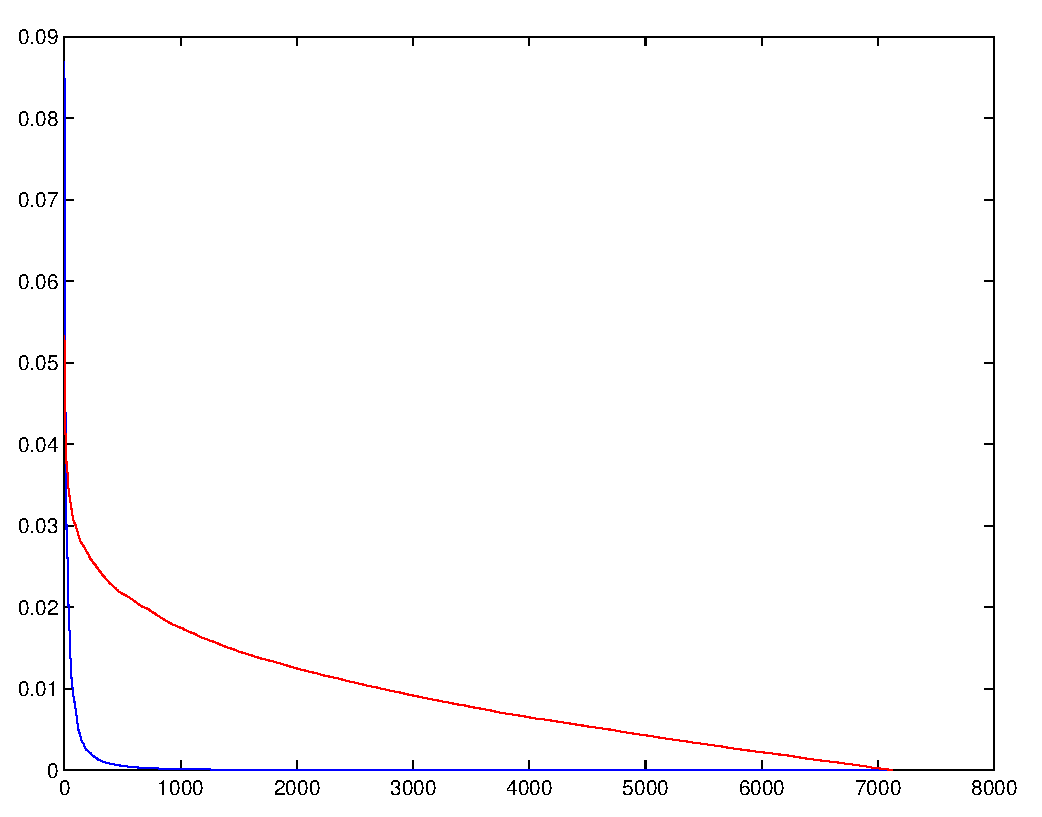
\includegraphics[scale=0.2]{featall.eps}
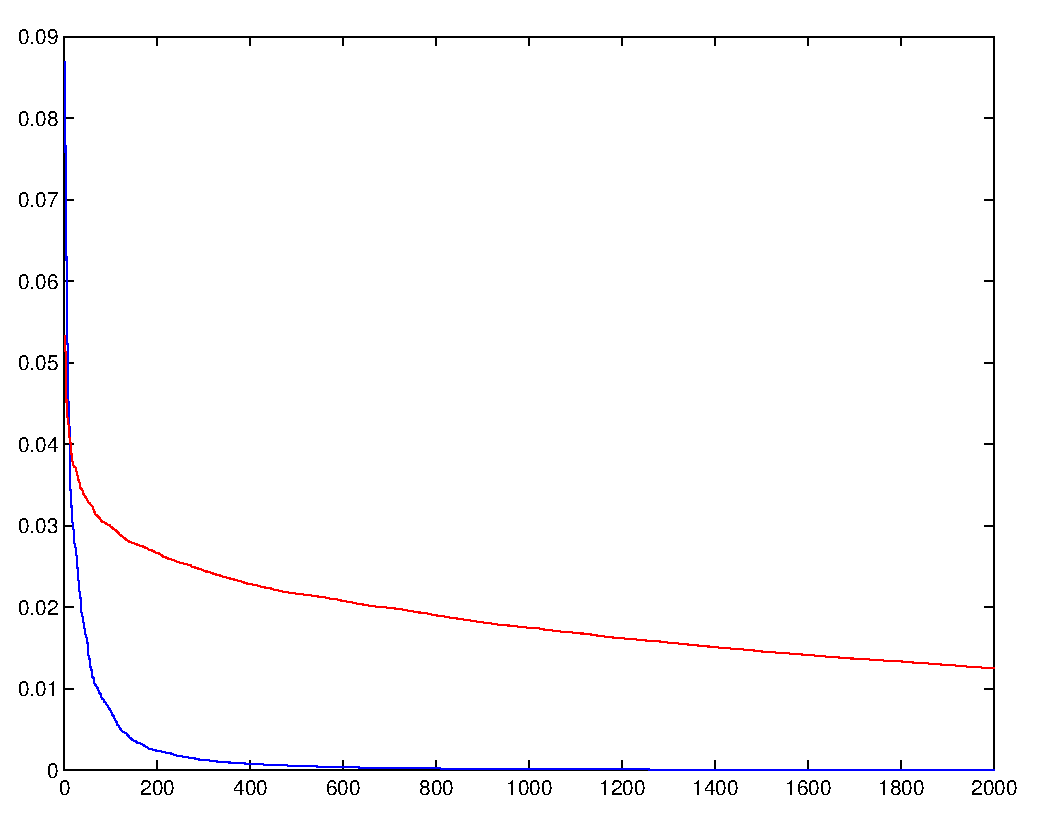
\includegraphics[scale=0.2]{feat2000.eps}
}
\vspace{.1in}
\centerline{
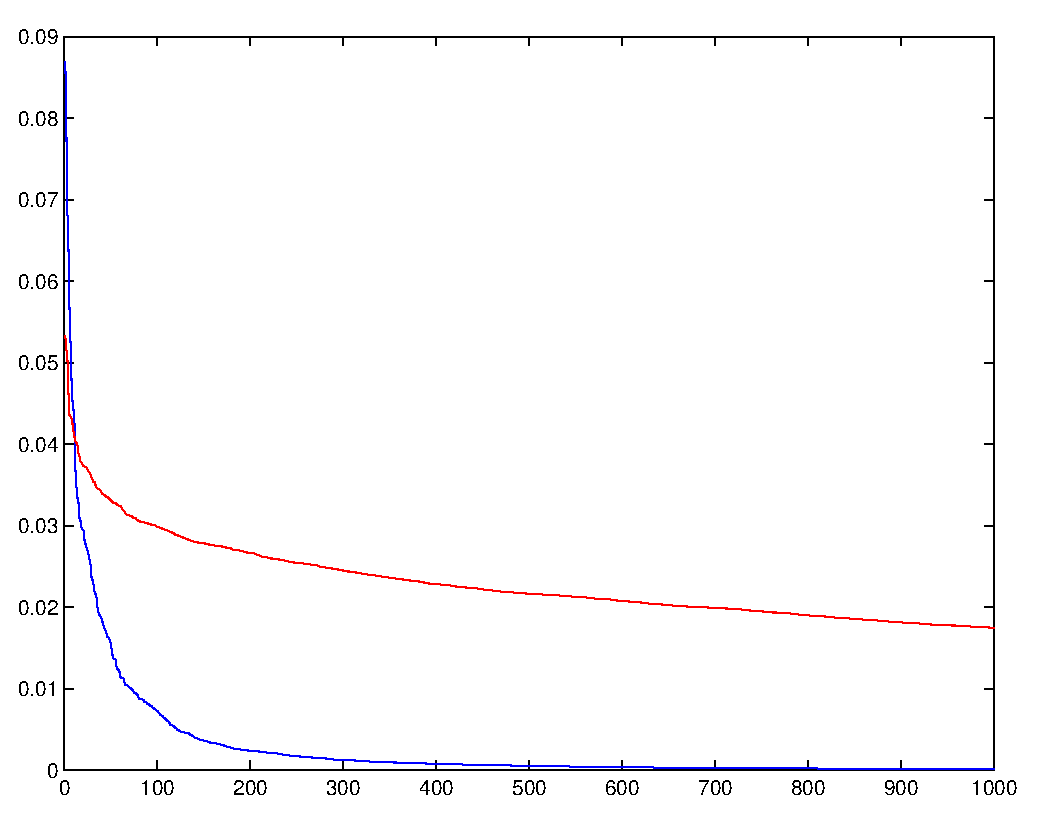
\includegraphics[scale=0.2]{feat1000.eps}
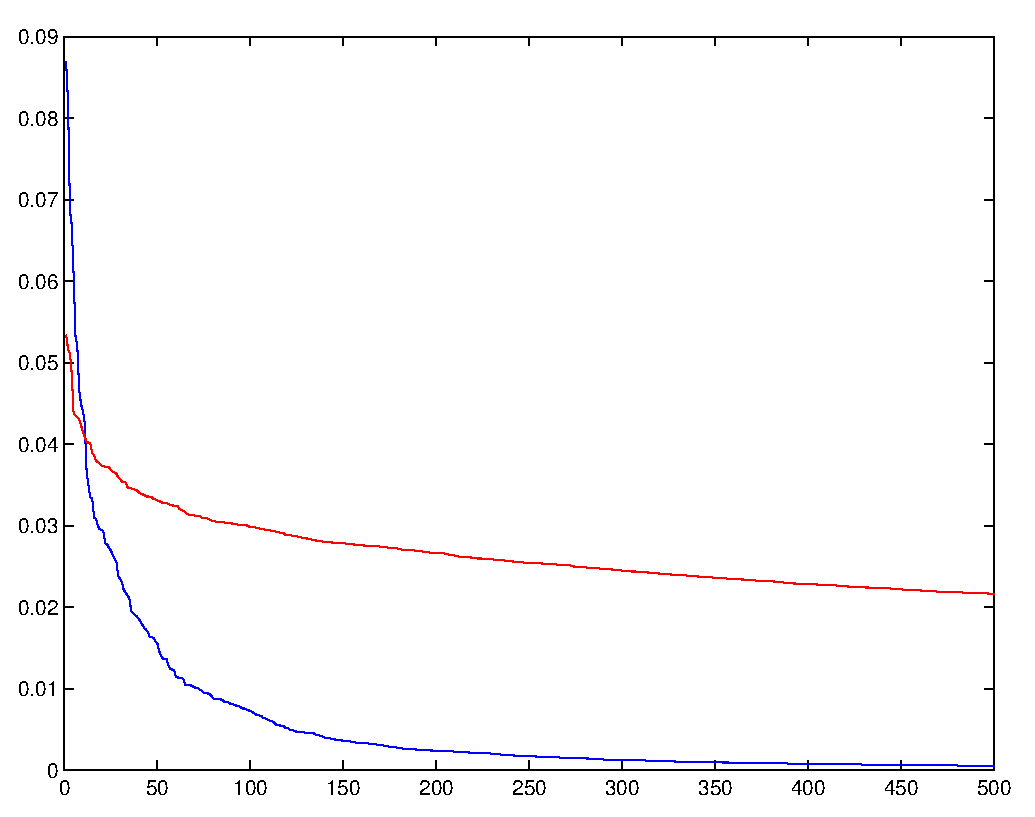
\includegraphics[scale=0.2]{feat500.eps}
}
\end{center}
}


}

\end{slide}

}


%-------------------------------------------------------------------- Slide --

\overlays{5}{
\begin{slide}{Discussion}

{\small

\fromSlide*{1}{
There are many extensions and refinements to this
method which we discuss below: 
\begin{itemize}


\item Logistic regression model: reduced matrix implementation and analysis
}

\fromSlide*{2}{
\item Fully Bayesian model: compute the full posterior using MCMC 
}

\fromSlide*{3}{
\item Intrinsic dimension: rate of convergence of the gradient has the
  form of $O(m^{-1/n})$, it would be good to replace $n$ with $n_{\cal M}$}

\fromSlide*{4}{
\item Semi-supervised setting: given ${\bf x}=(x_i)_{i=m+1}^{m + u}$
in addition to $\bf z$
\begin{eqnarray*}
\vec f_{\bz, {\bf x}, \gl, \mu} &=\arg\min_{\vec f \in\H_K^n}
\biggl\{\frac{1}{m^2}\sum_{i, j=1}^m w_{i, j}^{(s)}
\biggl(y_i-y_j+ \vec f (x_i)\cdot (x_j-x_i)\biggr)^2 \nonumber\\
&+ \frac{\mu}{(m +u)^2}\sum_{i, j=1}^{m+u} W_{i, j} |\vec f (x_i)-
\vec f(x_j)|_{\ell^2 (\rr^n)}^2 + \gl\|\vec f\|_K^2\biggr\},
\label{graregsemi}
\end{eqnarray*} 
where $\{W_{i, j}\}$ are edge weights in the data adjacency
graph, $\mu$ is another regularization parameter and often satisfies $\gl=o(\mu)$.
}

\end{itemize}

}


\end{slide}
}


%-------------------------------------------------------------------- Slide --

\begin{slide}{Acknowledgements}


{\small 
Andr\'e Elisseeff, Misha Belkin, Aravind Subramanian, Tommy Poggio,
and Steve Smale for discussions
}

\end{slide}


\end{document}
